\chapter{Introduction}

\section{Overview}

The project title contains two parts: a backend, and a service. The backend itself consists of three parts: a server, application, and a database. When booking a flight, the website you open known as the frontend is where the user enters their information. These customer’s information needs to be stored in a single location, so when the customer signs back in, their information still exists. This information is stored on a server in a database and logic to process this is known as a backend.

A service provides tools for mobile apps to interact with the backend. It is a way for developers to link their applications to backend cloud-based storage and services. A backend as a service or BaaS is best described by a tech analyst who refers to it as ''turn-on infrastructure'' for mobile and web apps. \cite{kinveywebsite}.

\section{Project Objectives}
The aim of this project is to develop a template for the development of mobile applications. This template is to help improve the development of modern mobile applications for new and experienced developers. The mobile backend as a service provides a selection of tools and services that enable rapid development of sophisticated mobile solutions. These services provided are given to help with the different phases of mobile app development. The project aim is to create a complete package that will enable new and experienced developers to speed up in the following areas:

\begin{enumerate}
  \item Development
  \item Testing 
  \item Production
\end{enumerate}

The project deliverables to aid with the three phases include the following:

\begin{enumerate}
   \item Mobile Back-end as a Service
  
    This is a model for developers to link their applications to the backend cloud storage and application programming interfaces (API's) exposed to provide the communication with the a list of services.
  \item Dashboard
  
    The dashboard is a control panel that simplifies configuring the web server. It also contains data visualization tools to monitor the mobile app's activity.
  \item iOS Framework
  
    The list of services need a way to communicate from back-end to the mobile apps. This is accomplish by providing a custom software development kits (SDKs). This provides the developer with native language communication.
\end{enumerate}

\section{System Overview}

\begin{figure}[h]
    \caption{Project Overview 2}
    \centering
    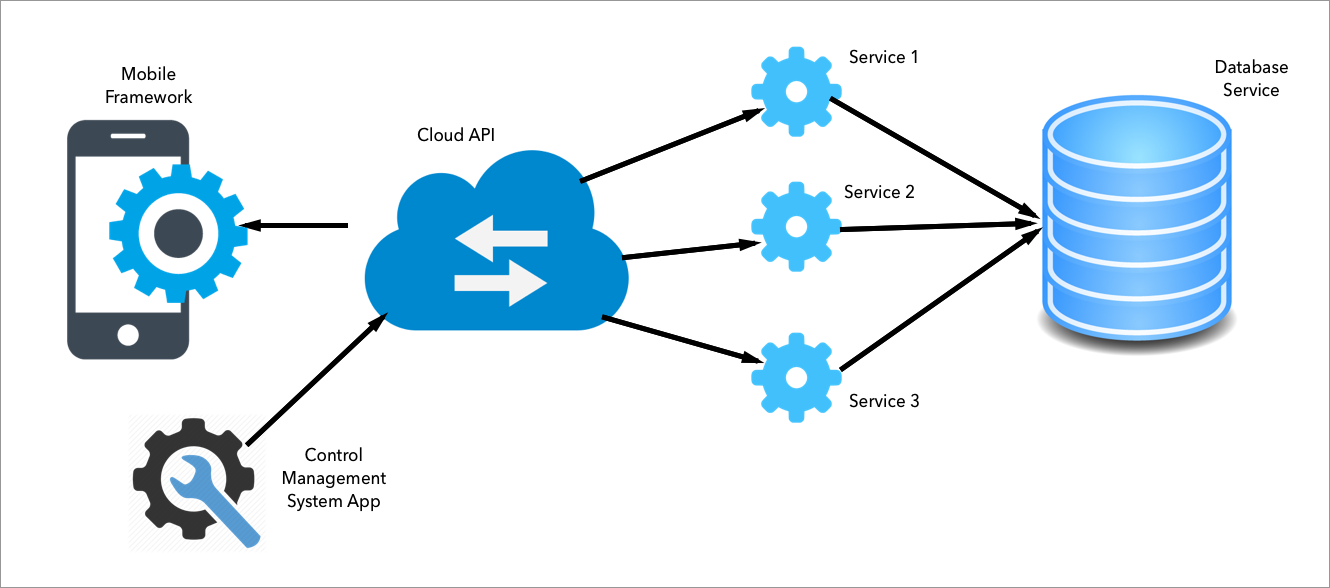
\includegraphics[width=100mm]{images/overview}
    \label{fig:project_overview1}
\end{figure}

\begin{figure}[h]
    \caption{Project Overview 2}
    \centering
    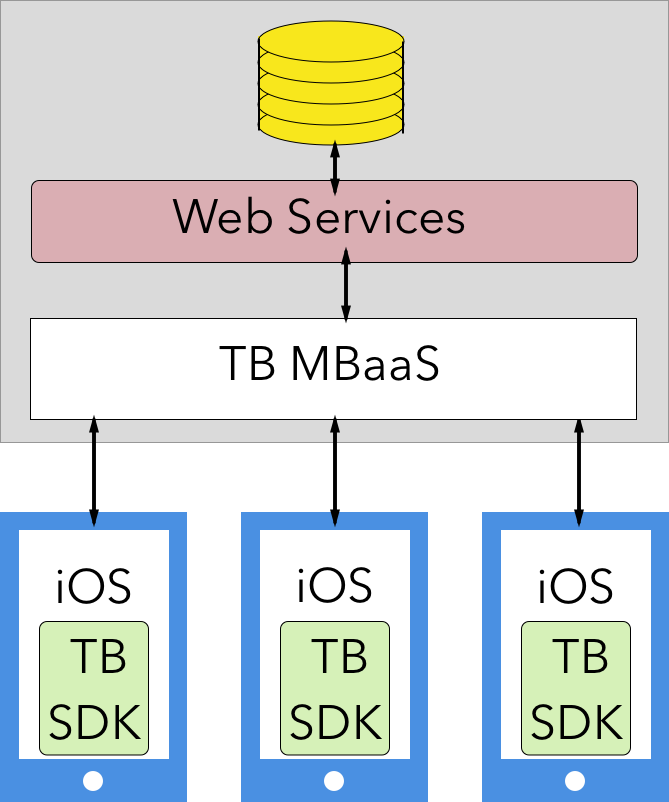
\includegraphics[width=60mm]{images/app_overview}
    \label{fig:project_overview2}
\end{figure}

The two Figures \ref{fig:project_overview1}, \ref{fig:project_overview2} illustrates the overall project overview. The Figure \ref{fig:project_overview1} shows the three deliverables and how they are connected to each other. In Figure \ref{fig:project_overview2} contains the iOS devices in which the SDK framework will reside. The backend containing the web sever with services and the database. 

\section{Project Challenges}

The key challenge of the project was to find what functional requirements developers are looking for when choosing a mobile backend as a service. This required asking question on mobile app forums and setting up meetings with professional mobile developers and getting their opinion on the project.

The biggest challenge faced was to find a way to enhance the developing stage of any application, giving more power to the developer when the application has been published. This lead to another challenge, to see how far Apple would allow applications to be configured after published.

\section{Chapter Walk-through}

\paragraph{Chapter 2 Research}

This chapters discusses the alternative existing solutions to the problem. It also goes into the potential technologies that could be used in the project along with the resultant findings. The technologies discussed will be what web server to use, the programming language and what the dashboard be development in. This chapter will include surveys and out-sourced discussions with professional mobile developers.

\paragraph{Chapter 5 Architecture}

The architecture chapter will show the overview diagram of the complete project, along with diagrams of the individual services.

\paragraph{Chapter 4 Design}

This chapters goes into the design of the project. What methodologies will be used?, and go into detail of the list of features required to complet this project achieved the goal.

\paragraph{Chapter 5 Development}

This chapter will discuses the different deliverables in the project in order to achieve the project aim. It will contain detail description of the features that will be used to aid in mobile application development.

\paragraph{Chapter 6 Implementation}

Implementation chapters explains how to use different deliverables included in the project. Along with code snippets which show how to set up the system and use the SDK.

\paragraph{Chapter 7 Testing/Evaluation}

This chapter will give an overview of all testing carried out including the test-driven approach and unit service testing. The evaluation section discusses the review given from the out-source professional developers. The review not only includes their feedback using the system but also their recommendations where to from here. 

\paragraph{Chapter 8 Conclusion}
The conclusion chapter contains a summary of the project overall and ends with a reflection of the project.

\paragraph{Appendices}
The conclusion chapter discusses the meetings and evaluations with out-sourced professional mobile app developers.